\section{Grouping Provenance graph nodes}  \label{sec:grouping}

%\comment{discuss (somewhere) implications of relaxing the assumption about connectivity in Section~\ref{sec:closure}.}



As mentioned in Sec.~\ref{sec:contributions}, our goal is to define graph editing operators that selectively remove information from a graph $G \in \guEA$, yielding a new graph $G' \in \guEA$.
%
The first of these, namely the removal of labels or annotations associated with a node or an edge, is straightforward. 
%
Regarding the removal of a node, we note that simply reconnecting the remaining nodes generally may lead to an invalid graph. 
%
A simple example is a graph defined by: $\{\used(a, e_1)$, $\wgby(e_2, a) \}$ where activity $a$ is removed. This results simply in two disconnected nodes $e_1$, $e_2$, because no relationship can be inferred between them from the original graph.


Rather than delving into the possible consequences of such node and edge elision, we are going to focus exclusively on the $\group$ graph transformation operator as the prime way to achieve abstraction over provenance graphs.
%
$\group$ takes a graph $G = (V, E) \in \guEA$ and a subset $V_{gr} \subset V$ of its nodes \jwb{that the user wishes to obfuscate} and produces a modified graph $G' \in \guEA$. The nodes in $V_{gr}$ are ``grouped'' together and replaced by a new single node.
%
  
\[ \group : \guEA \times \mathbb{P}(V) \rightarrow \guEA \]
  
%Here we define $\group$ over $\guEA$ graphs. This will be extended to abstraction over Agents in Sec.~\ref{sec:agents-abstraction}.

%The $\group$ operator has the following signature:

%
As the operator is closed under composition, further abstraction can be achieved by repeated grouping, either on multiple disjoint sets $V_{gr}$, or on sets that include abstract nodes (abstraction of abstraction).



%
To get a quick intuition of the  problems faced in the definition of the grouping operator, consider the transformation in Fig.~\ref{fig:non-convex-ex-1}, where nodes $V_{gr} = \{e_1, e_3, e_4, e_5\}$ are simply replaced with new node $e'$ in the example graph of Fig.~\ref{fig:baseline-ug-ae}, and all edges in and out of nodes in $V_{gr}$ are just ``rewired'' in and out of $e'$. 

\begin{figure*}
\centering
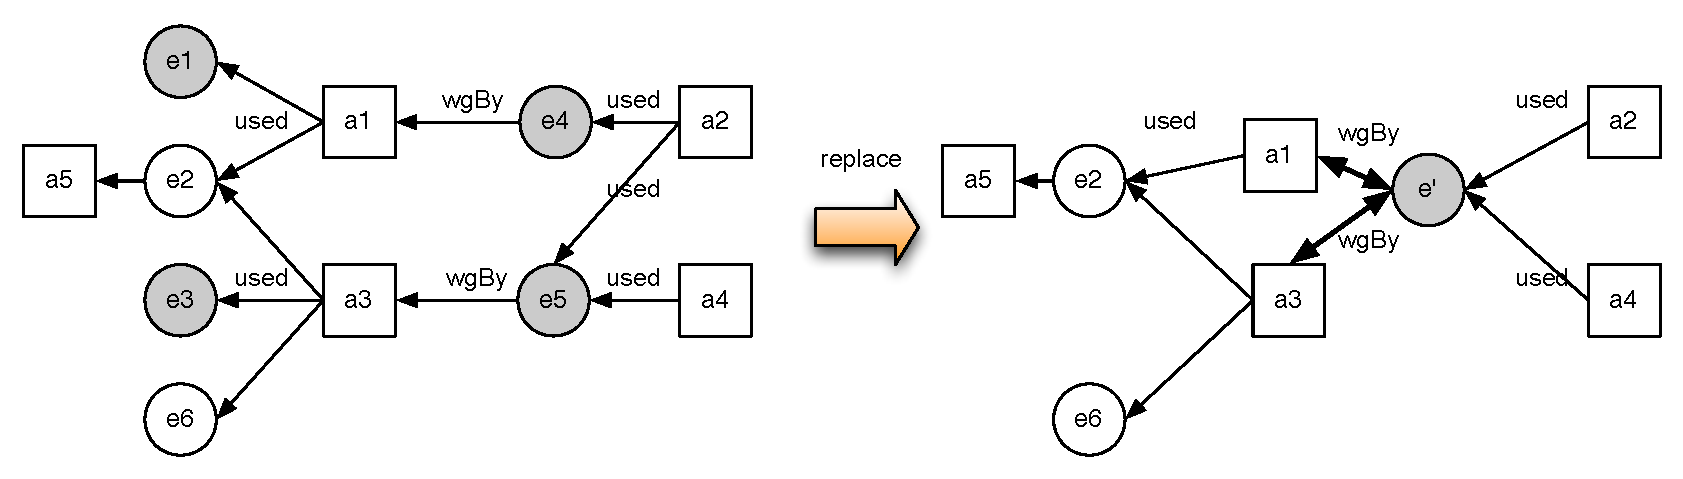
\includegraphics[scale=.5]{figures/non-convex-ex-1.pdf} 
\caption{Example: the careless abstraction of a set of nodes may lead to a non-$\guEA$ graph.} \label{fig:non-convex-ex-1}
\end{figure*}

This \jwb{illustrative example points out two problems.} Firstly, it introduces two cycles: $e'  \leftrightarrow a_1$ and $e'  \leftrightarrow a_3$. Furthermore, the two edges 
$e'  \leftarrow a_1$ and $e'  \leftarrow a_3$ cannot be of type $\wgby$, while at the same time one cannot arbitrarily introduce $\used$ relations, which would be false dependencies.
%the new node $e'$ appears to have been generated by two distinct activities, $a_1$ and $a_3$.
Thus, the resulting graph is not a valid PROV graph. Note that the former of these problems had been already pointed out in the description of the ProPub system~\citep{springerlink:10.1007/978-3-642-22351-8_13}, mentioned above.

\subsection{Closure and homogeneous grouping}
\label{sec:closure}

The example suggests that the \jwb{issue} is caused by nodes $a_1$ and $a_3$, which both lie on the paths between two of the nodes in $V_{gr}$. Intuitively, set $V_{gr}$ is not ``convex'', that is, there are paths in $G$ that lead out of $V_{gr}$ and then back in again. This observation suggests the introduction of a preliminary closure operation \textit{pclos}, which ensures acyclicity by capturing \jwb{and including these paths}. It is defined as follows.

%%%%
%% closure
%%%%
\vspace*{10pt}
\begin{definition}[Path Closure]
\label{def:clos}
Let $G = (V,E) \in \guEA$ be a provenance graph, and let $V_{gr} \subset V$.  
For each pair  $v_i, v_j \in V_{gr}$ such that there \jwb{one or more directed paths} $v_i \leadsto v_j$ in $G$, let $V_{ij} \subset V$ be the set of all nodes in \jwb{all paths $v_i \leadsto v_j$}.
The Path Closure of $V_{gr}$ in $G$ is
\[\clos(V_{gr}, \jwb{G})  =  \bigcup_{v_i, v_j \in V_{gr}} V_{ij} \]
\end{definition}

\jwb{We assume, for the moment, that the subgraph given by $\clos(V_{gr}, G)$ is a subgraph of $G$ with the property that each source is connected to at least one of the sinks. For now, we assume there is only one such subgraph that contains all the nodes in $V_{gr}$. 
}

%\jwb{ connected graph. In Section~\ref{sec:allowing} we explore the implications of relaxing this assumption.}  \comment{Check consistency with 4.3}



\begin{figure*}
\centering
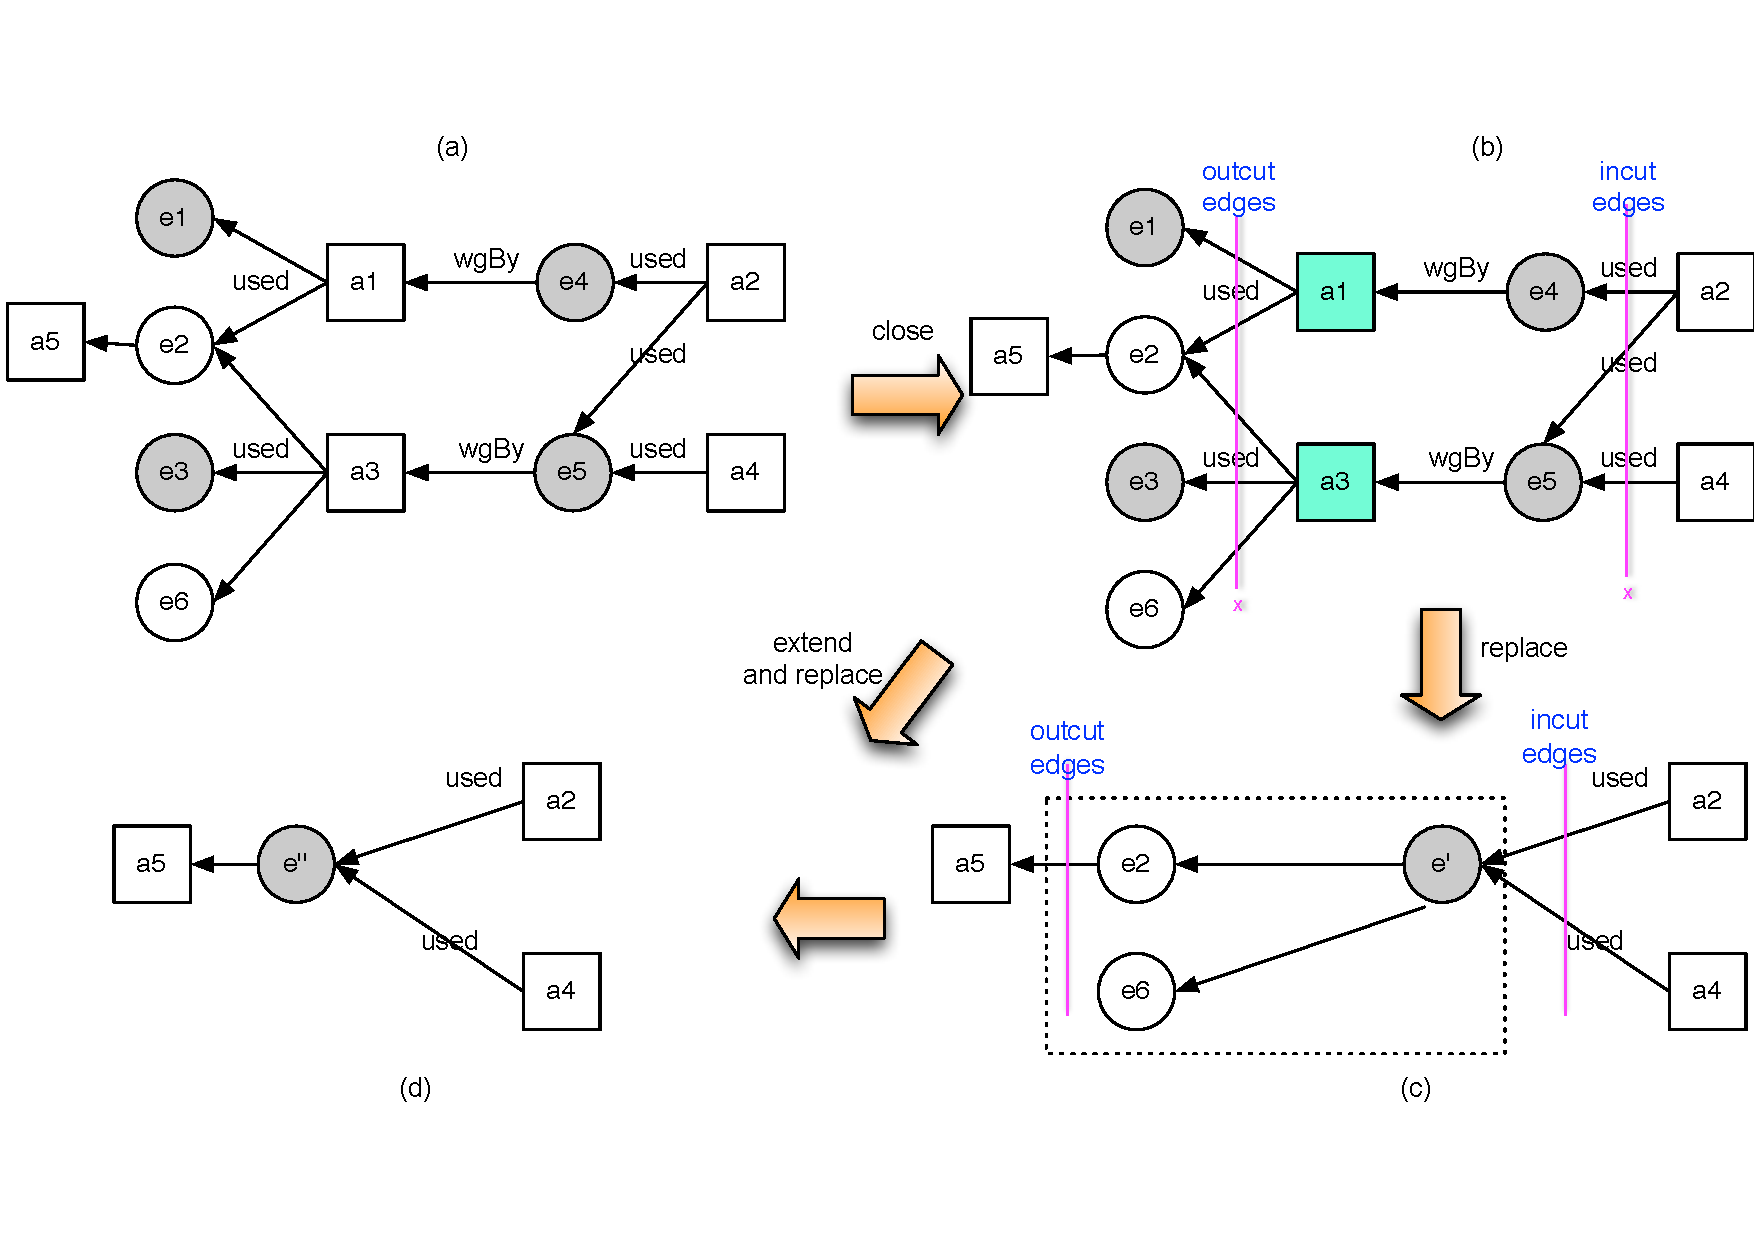
\includegraphics[scale=.5]{figures/convex-ex-1-revision.pdf} 
\caption{Path closure and replacement with extension on a set of entity nodes.} \label{fig:convex-ex-1}
\end{figure*}

Fig.~\ref{fig:convex-ex-1} shows a continuation of the previous example. This time the replacement is performed on $\clos(\{e_1, e_3, e_4, e_5\},G) = \{e_1, e_3, e_4, e_5, a_1, a_3\}$, \jwb{(in Fig.}~\ref{fig:convex-ex-1}(b)),  resulting in graph \jwb{in Fig.~\ref{fig:convex-ex-1}(c).}
%
However, while this solves the cycle problem, the graph is no longer bipartite, \jwb{because} the new edges $e' \rightarrow e_2$ and $e' \rightarrow e_6$ connect nodes of the same type.
%
In this example, we can construct a new group of nodes, $\{ e', e_2, e_6\}$, on the graph that results from the first replacement, and replace it with a new node $e''$. The resulting graph \jwb{Fig.~\ref{fig:convex-ex-1}(d)} is a valid $\guEA$ graph.

%
The same result can be obtained by first \textit{extending} the closure in \jwb{Fig.~\ref{fig:convex-ex-1}(b)} to include e-nodes $e_2$, $e_6$, and then replacing the resulting set with $e''$ (this is indicated by the ``extend and replace'' arrow from \jwb{Fig.~\ref{fig:convex-ex-1}(b)} to \jwb{Fig.~\ref{fig:convex-ex-1}(d) as} shown).
%
\jwb{The $\extend$ operator will have the role of ``gathering up'' certain nodes into the set to be replaced, and the purpose of $\extend$ is to ensure that the eventual node replacement preserves the type-consistency of graph.}
\jwb{We require all the set boundary nodes (nodes connected to nodes not in the set) to be of the same type, so in Fig.~\ref{fig:convex-ex-1}(b) we must  include nodes $e_2$ and $e_6$.}

Following this approach, we are going to define grouping as a composition of three functions: \textit{closure}, defined above, \textit{extension}, and \textit{replacement}, as follows.

%
The \textit{extension} of a set $V_{gr} \subset V$ relative to type $t \in \{ \en, \act \}$ is $V_{gr}$ augmented with all its adjacent nodes, in either direction, of type $t$. %\jwb{We do this because when we later replace this extended set with a single abstract node of type $t$, we want to ensure that we maintain type-correctness of the graph.}
Formally:


%%%%
%% extension
%%%%
% \vspace*{10pt}
% \begin{definition}[$\extend$]
% Let $G = (V,E) \in \guEA$, $t \in \{ \en, \act \}$.
% \[
% \begin{array}{l}
% \extend(V_{gr}, G ,t) =  \\
% \quad V_{gr} \;\cup \\ 
% \quad    \{ v' | (v \leftarrow v') \in E \wedge v \in V_{gr} \wedge \type(v') = t \} \;\cup \\
% \quad   \{ v | (v' \leftarrow v) \in E \wedge v \in V_{gr} \wedge \jwb{\type(v) = t} \}  \\
% \end{array}
% \]
%\end{definition}
%\comment{The nodes we to which we extend must have the type $t$. It isn't possible to include a node of type other than t.}

\comment{To make the defn below more clear, we use $v_s,v_d \nin V_{gr}$ in the definition of $extend$. This will also make this definition more compatible with the definitions of incut and outcut.}


\vspace*{10pt}
\begin{definition}[$\extend$]
  \label{def:extend}
  Let $G = (V,E) \in \guEA$, $t \in \{ \en, \act \}$. $v_s$ and $v_d$ are the source and destination nodes of a relationship.
  %\comment{we could replace $V_{gr}$ in the defn below with something that suggests $\clos$ has been applied?}
\[
\begin{array}{l}
\extend(V_{gr}, G ,t) =  \\
\quad V_{gr} \;\cup \\ 
\quad    \{ v_d | (v_d \leftarrow v_s) \in E \wedge v_s \in V_{gr} \jwb{~\wedge\ v_d \nin V_{gr}} \wedge \type(v_d) = t \} \;\cup \\
\quad   \{ v_s | (v_d \leftarrow v_s) \in E  \jwb{~\wedge\ v_s \nin V_{gr}} \wedge v_d \in V_{gr}  \wedge \jwb{\type(v_s) = t} \}  \\
\end{array}
\]


\end{definition}

\comment{I've replaced the phrase ``sink node'' with ``boundary node'' in the following.}

%
In our example, $\extend(\{e_1, e_3, e_4, e_5, a_1, a_3\}, G, \en) = \{e_1, e_3, e_4, e_5, a_1, a_3, e_2, e_6\}$.  Note that all boundary nodes in $\extend(V_{gr}, G, t)$ are of type $t$ by construction.
%\footnote{A boundary node is any node in the extended set with a link to a node not in the set.}

Next, we  \jwb{replace} the collected nodes with a new abstract node.
%
Let $V^* \subset V$ be obtained using $\pclos$ then $\extend$, as outlined above, and let $v_{new}$ be a new node  that does not appear in $V$.
%
Function $\repl$ replaces $V^*$ with $v_{new}$ in $V$, and connects $v_{new}$ to the rest of the graph.
\jwb{To aid us in the definition, we begin by defining the \textit{outcut}, \textit{incut} and the \textit{internal} nodes of $V^*$.}

Let $\vartheta_{out}(V^*)$ denote the \textit{outcut} of $G$ associated with $V^*$, defined as:
\jwb{\[ \vartheta_{out}(V^*) = \{  (v_d \leftarrow v_s) |   v_s \in  V^*, v_d \in V \setminus V^*\}\]}
This is the set of arcs of $G$ pointing out of $V^*$.
%
Symmetrically, let $\vartheta_{in}(V^*)$ denote the \textit{incut}  of $G$ associated with $V^*$, i.e., the set of arcs of $G$ leading into $V^*$:
\jwb{\[ \vartheta_{in}(V^*) = \{  (v_d\leftarrow v_s) |  v_d \in V^*, v_s \in  V \setminus V^* \}\]}
%
Finally, let $\vartheta_{int}(V^*)$ denote internal arcs, that connect two both nodes inside $V^*$:
\[ \vartheta_{int}(V^*) = \{  (v_s\leftarrow v_d) | v_s, v_d \in V^*\}\]


\jwb{Function $\repl$ replaces each arc $(v_d \leftarrow v_s) \in \vartheta_{out}(V^*)$ with a new arc $(v_{d} \leftarrow v_{new})$ of the same type, and replaces each arc $(v_d \leftarrow v_s) \in \vartheta_{in}(V^*)$ with a new arc $(v_{new} \leftarrow v_{d})$ of the same type. Arcs in $\vartheta_{int}(V^*)$ simply disappear along with the nodes in $V^*$.}
%


%
\jwb{The definitions of $\vartheta_{out}'(V^*)$ and $\vartheta_{in}'(V^*)$ below define the final part of the ``rewiring'' carried out by $\repl$. }

\begin{definition}
  Let $ty \in \{\used,  \wgby\}$. Then:
  \begin{align*}
\vartheta_{out}'(V^*) = \{ & \jwb{(}v \xleftarrow{ty}  v_{new} \jwb{)}|  v \xleftarrow{ty} v' \in \vartheta_{out}(V^*)  \}  \\
\vartheta_{in}'(V^*) = \{ & \jwb{(}v_{new} \xleftarrow{ty} v \jwb{)} | v' \xleftarrow{ty} v \in \vartheta_{in}(V^*)  \}   
\end{align*}
\label{def:eq:outcut}
\end{definition}

% \begin{align}
% \vartheta_{out}'(V_{gr}') = \{ & v \xleftarrow{t}  v_{new} |  v \xleftarrow{t} v' \in \vartheta_{out}(V_{gr}')  \}  \\
% \vartheta_{in}'(V_{gr}') = \{ & v_{new} \xleftarrow{t} v | v' \xleftarrow{t} v \in \vartheta_{in}(V_{gr}')  \}   \label{eq:outcut}
% \end{align}
% 

\noindent
\jwb{And the full definition of $\repl$ is}
\vspace*{10pt}
\begin{definition}[replace]
\label{def:group-replace}

\[ \repl (V^*, v_{new}, G) = (V', E'), \mbox{ where: } \]
\begin{eqnarray*}
V' & = & V  \setminus V^*  \cup \{v_{new}\}\\
E' & = & E  \setminus (\vartheta_{out}(V^*) \cup \vartheta_{in}(V^*) \cup \vartheta_{int}(V^*))  \\
   & & \qquad \cup\  \vartheta_{out}'(V^*)  \cup \vartheta_{in}'(V^*)
\end{eqnarray*}
% \begin{align*}
% V' = V & \setminus V_{gr}  \cup \{v_{new}\}\\
% E' = E & \setminus (\vartheta_{out}(V_{gr}) \cup \vartheta_{in}(V_{gr}) \cup \vartheta_{int}(V_{gr}))  \\
%     & \cup \vartheta_{out}'(V_{gr})  \cup \vartheta_{in}'(V_{gr})
% \end{align*}
\end{definition}

It is easy to verify that the resulting graph is type-correct. All boundary nodes in \jwb{$V^*$}  are of the \jwb{same type $t \in \{En,Act\}$,} as noted above, and   $v_{new}$ \jwb{is of type $t$}  by construction.
%Thus, boundary nodes are replaced by a node $v_{new}$ of the same type.
Since the arcs have the same type as those they replace, it follows that $\repl$ preserves type correctness.



\begin{figure*}
\centering
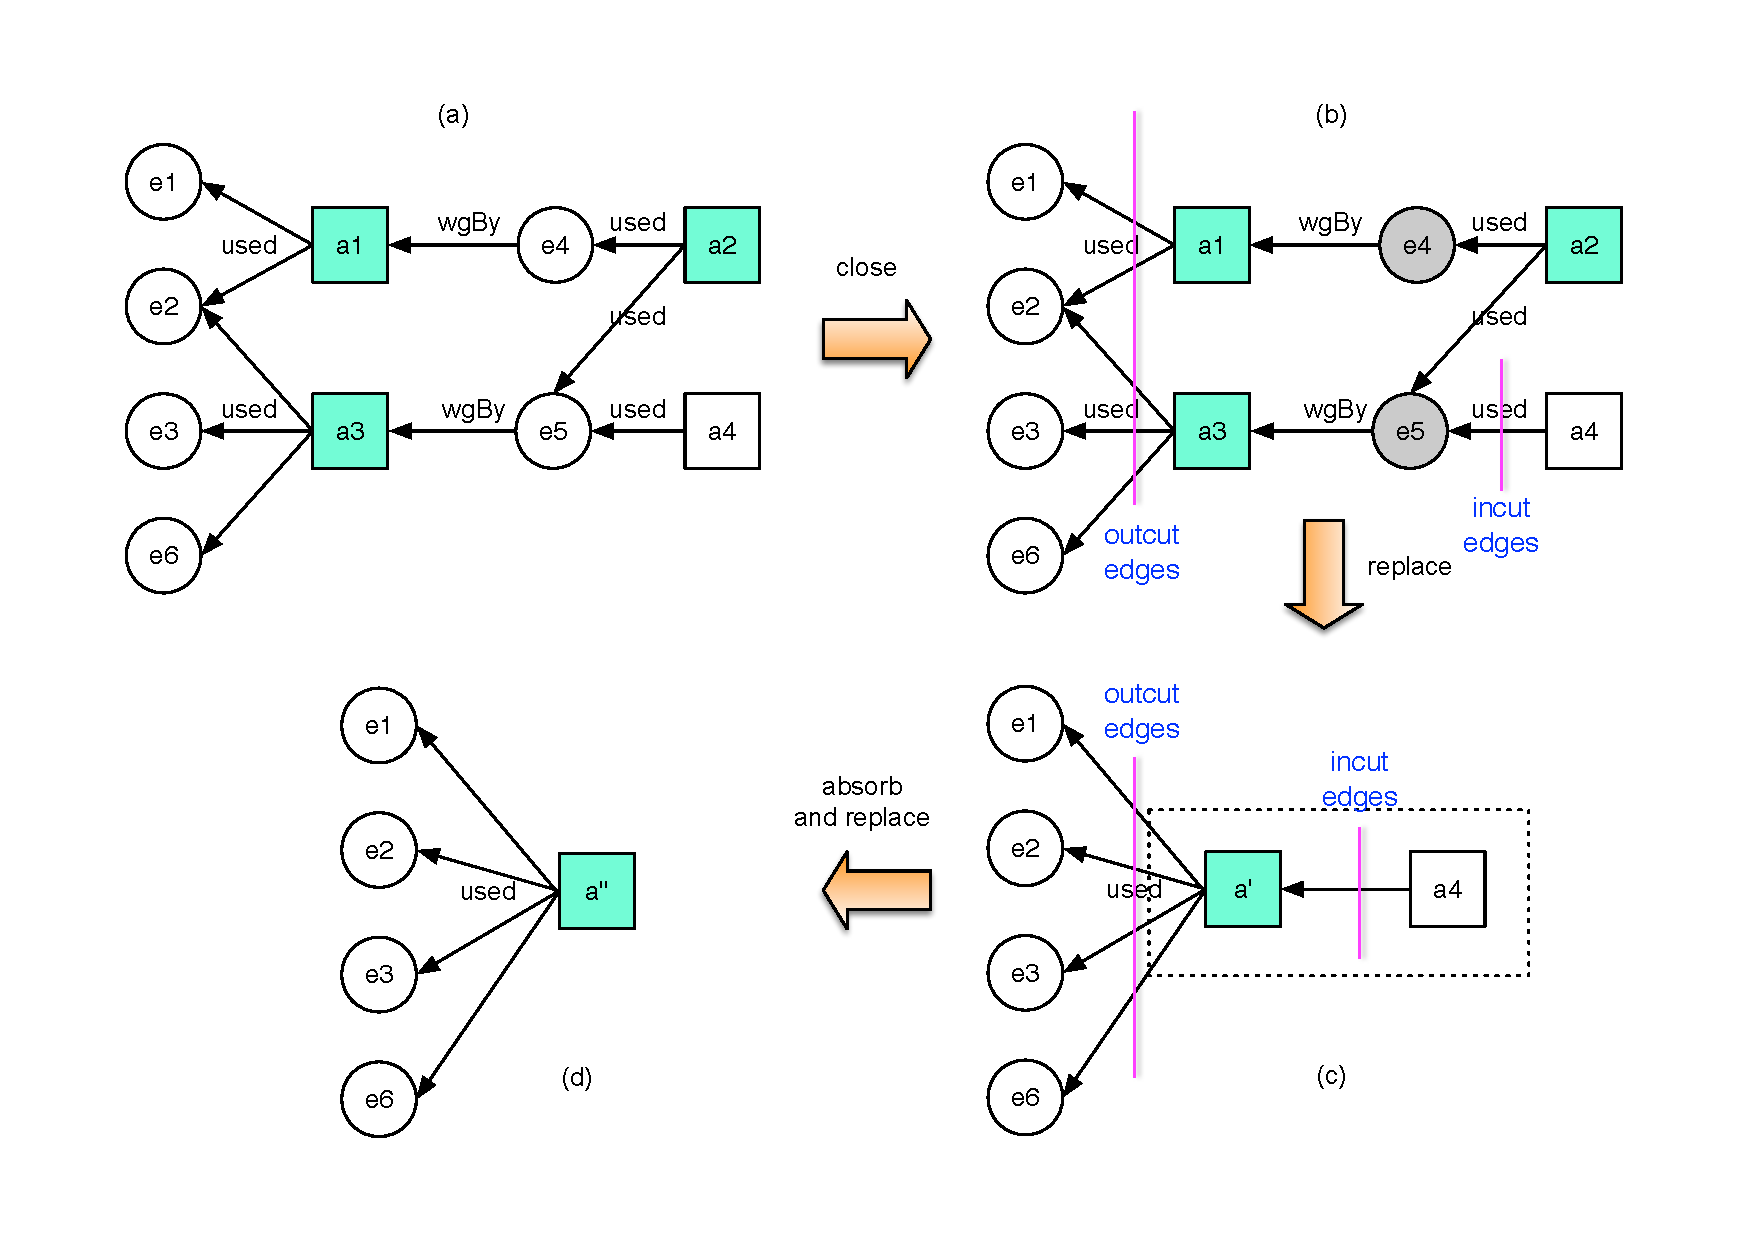
\includegraphics[scale=.5]{figures/convex-a-only-revision.pdf} 
\caption{Grouping on a set of Activity nodes} \label{fig:convex-a-only}
\end{figure*}

We can now provide an initial definition of our $\group$ operator, under the simplifying assumption that all nodes in $V_{gr}$ are of the same type \jwb{before closure.}  We denote this type by $\type(V_{gr})$ (with a slight abuse of notation). \jwb{Definitions~\ref{def:t-grouping} and~\ref{def:strict-t-grouping}  in Section~\ref{sec:generalisation} remove this asumption.}

Fig.~\ref{fig:convex-a-only} shows a progression similar to that of Fig.~\ref{fig:convex-ex-1}, but this time $\type(v) = \act$ for each $v \in V_{gr} = \{a_1, a_2, a_3\}$, and $V_{gr}$ is replaced by another activity node, $a'$.
%
Under assumption of type homogeneity, the grouping operator is a functional composition of $\clos$, $\extend$, and $\repl$ functions, defined as follows.

\vspace*{10pt}
\begin{definition}[Homogeneous Grouping]
Let $G=(V,E) \in \guEA$, $V_{gr} \in V$ be a type-homogeneous set, and let $v_{new}$ be a new node with $\type(v_{new}) = \type(V_{gr})$.
\begin{align*}
\group_{hom} &  (G, V_{gr}, v_{new}) = \\
 & \repl(  \\
 & \extend( \\
 & \clos(V_{gr},\jwb{G}), V, \type(V_{gr})), v_{new},  G ) 
\end{align*}
\label{def:homo-group}
\end{definition}

As an illustration, in our running example in Figure~\ref{fig:convex-ex-1} we have: %Ive altered this example: see latex for orig.
\begin{align*}
V_{gr} &= \{e_1, e_3, e_4, e_5\} \\
V_{cl} & = \clos(V_{gr},G) = \{e_1, e_3, e_4, e_5, a_1, a_3\} \\
V^{*} & = \extend(V_{cl}, \en) = V_{cl} \cup  \{e_2, e_6 \} \\
\group_e(G, V_{gr}, v_{new}) & = \repl(V^{*}, v_{new}, G) \\
& = (\{a_1,a_2,a_3,e''\}, \{ (a_2, e''), (a_4, e''), (e'',a_5) \})
\end{align*}



%\jwb{\subsubsection{Summary}}

\jwb{In this section we have described the grouping operator in terms of the component functional parts.}
\jwb{Up to this point we have been operating under the assumption made in Definition~\ref{def:clos}: that there is only one subgraph generated  by  $\clos(V_{gr}, G)$.  In the case where we have two or more subgraphs,  the $\extend$ operator and the $\repl$ operator would iterate over these sets, and by applied to each subgraph separately. }
\jwb{A further assumption, that all nodes in the initial selected set are the same type, is dealt with in the following  Section.}


\subsection{Generalization to \textit{e-grouping} and \textit{a-grouping}}
\label{sec:generalisation}

So far we have considered grouping over sets $V_{gr}$ of type-homogeneous nodes (before closure). Additional care must be taken if we allow $V_{gr}$ to include nodes of mixed types.  The type of the replacement node must now be specified, as it is no longer implied from the type of the nodes in $V_{gr}$. Indeed, the choice of such type leads to different abstracted graphs. Thus, we will now refer to grouping as \textit{t-grouping}, where $t \in \{ \en, \act\}$, i.e., \textit{e-grouping} or \textit{a-grouping}. Fig.~\ref{fig:e2-a4}(a-1, a-2) illustrates the application of the $\group_{hom}$ operator (Def.~\ref{def:homo-group}), assuming \textit{a-grouping} and $V_{gr} = \{ e_4, a_2\}$. Because the boundary nodes for the set to be replaced must be of type activity, the extension incorporates activity node $a_1$.



%\jwb{As an illustration, observe that \textit{e-grouping} and \textit{a-grouping} lead to different patterns in  Fig.~\ref{fig:e2-a4}(e-1, e-2).}

\jwb{Consider now the case of \textit{e-grouping} in Fig.~\ref{fig:e2-a4}(e-1, e-2).}  \comment{Not sure why the nodes are different colours?. Shape and label are together  sufficient indicators of type. The colours could indicate the actions of $\pclos$, extend and replace?} \comment{Also, I think we should replace the gXXand uXX labels with used and wgBy for consistency with the previous diagrams.}
%
Now the extension leads to $V_{cl} = V_{gr} \cup \{ e_5\}$, which in turn leads to the pattern shown in Fig.~\ref{fig:e2-a4}(e-2), involving two generation events for the new entity $e_{N}$.

Although this is a valid pattern, the two generation events must be simultaneous (this is one of the temporal constraints defined in~\citep{w3c-prov-constraints}):
\begin{align*}
ev(\wgby(e_N, a_1)) & \preorder ev(\wgby(e_N, a_3))  \quad \wedge \\
ev(\wgby(e_N, a_3)) & \preorder ev(\wgby(e_N, a_1))
\end{align*}

The intuitive interpretation for this pattern is that each of the two activities generated one entity in the group represented by $e_N$, and that the abstraction makes these two events indistinguishable. Formally, nothing further needs to be done to the graph. \jwb{We will explore the implications of the event ordering rules further in Section~\ref{sec:event}.  }  However note that one can restore, if desired, the more natural pattern whereby one single generation event is recorded for $e_N$. This is achieved simply by propagating the grouping to the set of generating activities. In the example, this leads to the graph in Fig.~\ref{fig:e2-a4}(e-3).  



\begin{figure*}
\centering
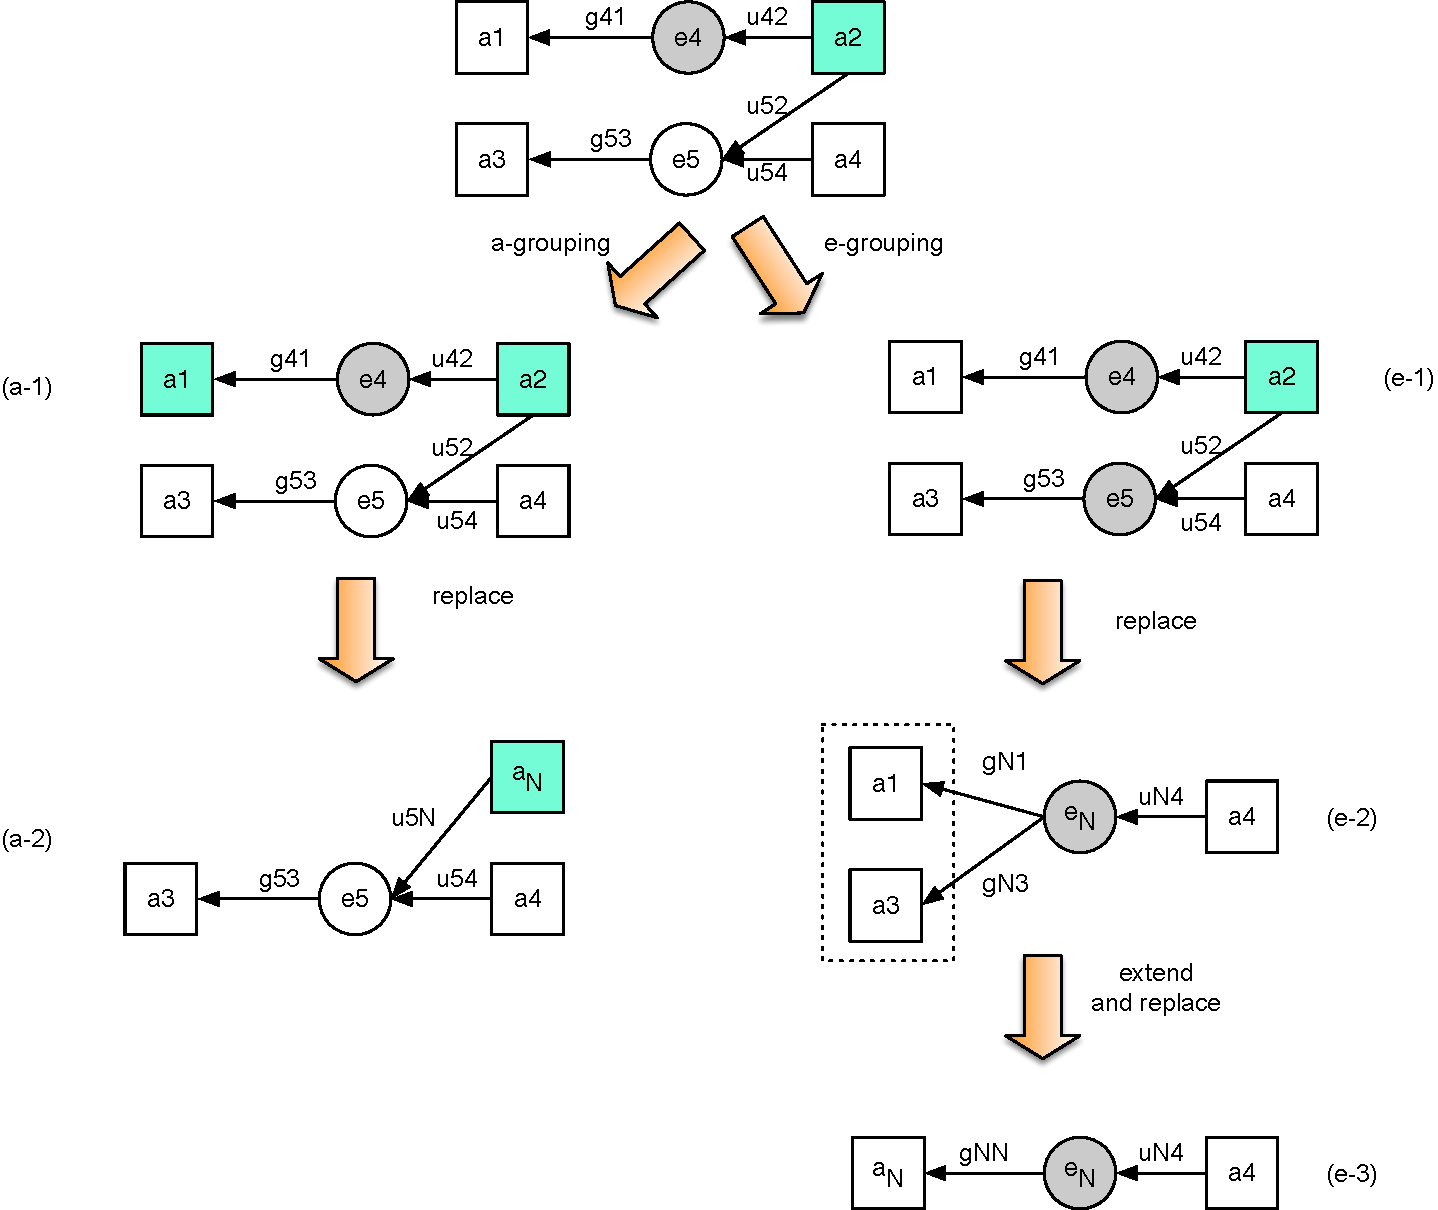
\includegraphics[scale=.5]{figures/e2-a4.pdf} 
\caption{e-grouping and a-grouping on mixed type nodes} \label{fig:e2-a4}
\end{figure*}

We now formalize these considerations by introducing two definitions for $\group$. The first, which we call \textbf{t-grouping}, is agnostic of multiple generation patterns, while the second (\textbf{strict t-grouping}) applies propagation to ensure that the graph is free from multiple generation patterns.

\vspace{10pt}
\begin{definition}[t-Grouping]
\label{def:t-grouping}
Let $G=(V,E) \in \guEA$, $V_{gr} \in V$, $t \in \{\en, \act\}$, and let  $v_{new}$ be a new node with $\type(v_{new}) = t$.
%
Then:
\begin{align*} 
\group & (G, V_{gr}, v_{new}, t) = \\
& \repl( \extend(\clos(V_{gr},\jwb{G}), V, t), v_{new},  G )
\end{align*}
\label{eq:t-grouping}
\end{definition}

Note that the assumption that \jwb{boundary} nodes in the closure are homogeneous and are replaced by a node of the same type $t$, which is necessary for $\repl$ to perform correctly, still holds in this case. 

\begin{definition}[Strict t-Grouping]
Given 
$G=(V,E) \in \guEA$, $V_{gr} \in V$, $t \in \{\en, \act\}$, and a new node $v_{new}$ with $\type(v_{new}) = t$, let
\[ G' = (V',E') = \group(G, V_{gr}, v_{new}, t). \]
Let 
$V_{gen} = \{ a \in V' |  a \xleftarrow{\wgby} v_{new} \in E' \}$ be the set of activity nodes that generate $v_{new}$ according to $G'$, and let $a_{new}$ be a new activity node. Then:
\begin{equation*}
%\footnotesize
\sgroup(G, V_{gr},v_{new}, t)=
\begin{cases}
G' & \!\text{if}  |\!V_{gen}\!| \leq 1  \\
\repl(V_{gen}, a_{new}, G') & \!\text{otherwise } 
\end{cases}
%\normalsize
\end{equation*}
\label{def:strict-t-grouping}
\end{definition}

% \begin{align*}
% \sgroup & (G, V_{gr},v_{new}, t)=\\%
% & \begin{cases}
%     G' & \!\text{if}  |\!V_{gen}\!| \leq 1  \\
%     \repl(V_{gen}, a_{new}, G') & \!\text{otherwise } 
%   \end{cases}
% \end{align*}
% 
% 

%\jwb{if a1 and a3 were linked via an intermediate entity node, would this be a problem?}

It is straightforward to show that strict t-grouping reduces to normal grouping if the grouping is a homogeneous a-grouping:
\begin{align*}
&\text{if } \type(t) =  \act \\
 &\qquad\text{then } \sgroup(G, V_{gr},t) = \group(G, V_{gr},t). 
\end{align*}


%
%
%In addition, however, they are also subject to ordering constraints relative to events associated to elements in in $V_{cl}$ (the set of nodes to be grouped, resulting from Path Closure on source graph $G'$), which have now been replaced by the grouping nodes. To illustrate this reasoning, consider for instance the simple graph in Fig.~\ref{fig:simple-prototype-pattern-events}(a), and let $V_{gr}= \{ e_1, e_2\}$. The ordering constraints on $G$ are as follows:
%
%
%\begin{figure}
%\centering
%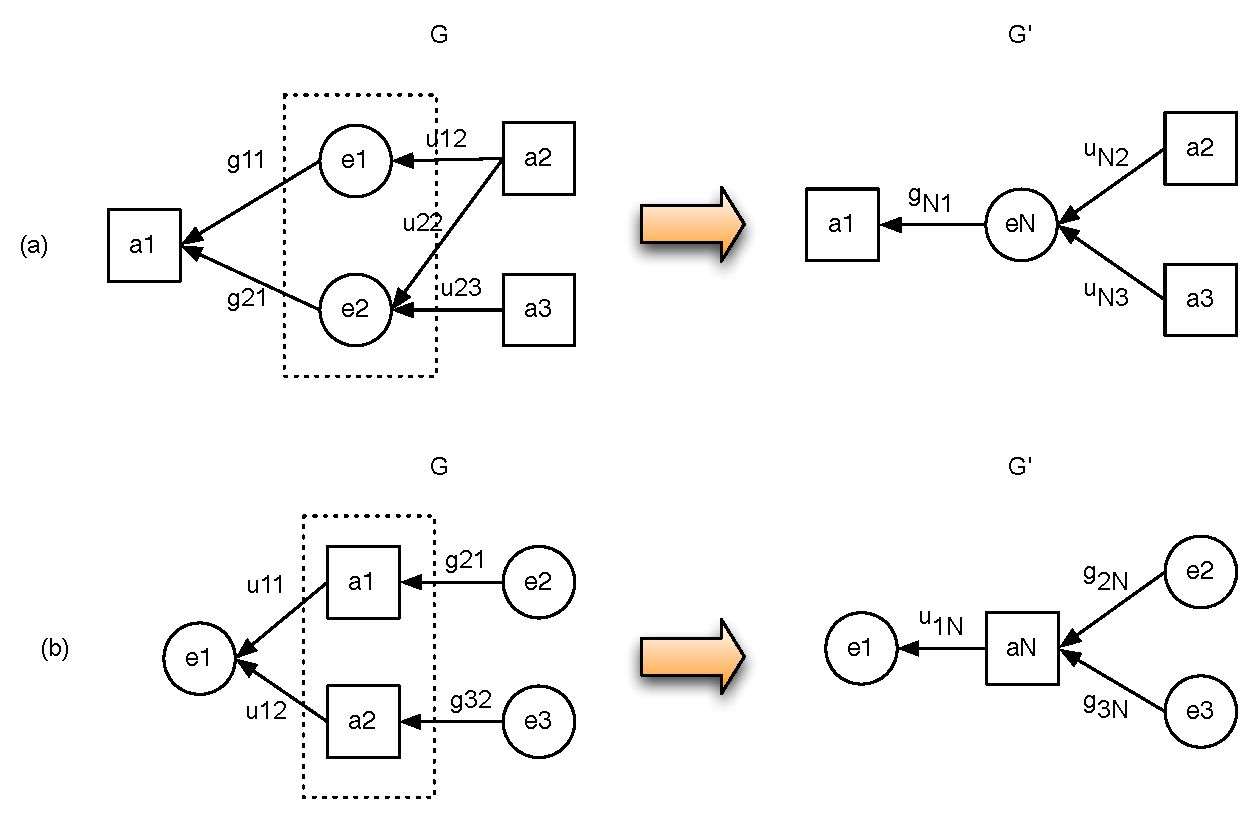
\includegraphics[scale=.5]{figures/simple-prototype-pattern-events} 
%\caption{Simple graph patterns to illustrate ordering constraints on events after grouping} \label{fig:simple-prototype-pattern-events}
%\end{figure}
%
%
%\begin{align*}
%start_{ev}(a_1) \preorder gen_{ev}(\wgby(e_i, a_1)) \preorder end_{ev}(a_1)   \text{ for } i=1, i=2\\
%start_{ev}(a_2) \preorder usage_{ev}(\used(a_2,e_1)) \preorder end_{ev}(a_2) \\
%start_{ev}(a_j) \preorder usage_{ev}(\used(a_j,e_2)) \preorder end_{ev}(a_j) \text{ for } j=2, j=3 \\
%gen_{ev}(\wgby(e_2, a_1))  \preorder usage_{ev}(\used(a_j,e_2))  \text{ for } j=1, j=2 \\
%gen_{ev}(\wgby(e_1, a_1))  \preorder usage_{ev}(\used(a_2,e_1)) \\
%\end{align*}
%%
%The corresponding ordering constraints on $G'$ are as follows.
%%
%\begin{align}
%start_{ev}(a_1) \preorder gen_{ev}(\wgby(e_N, a_1)) \preorder end_{ev}(a_1)  \label{eq:constraints-example-1}  \\
%start_{ev}(a_2) \preorder usage_{ev}(\used(a_2, e_N)) \preorder end_{ev}(a_2) \\
%start_{ev}(a_3) \preorder usage_{ev}(\used(a_3, e_N)) \preorder end_{ev}(a_3) \\
%gen_{ev}(\wgby(e_N, a_1))  \preorder usage_{ev}(\used(a_2,e_N)) \\
%gen_{ev}(\wgby(e_N, a_1))  \preorder usage_{ev}(\used(a_3,e_N)) \label{eq:constraints-example-n} 
%\end{align}
%
%The following additional ordering constraints further characterize events in $G'$ in terms of events in $G$. It is easy to see that such constraints are sufficient conditions for the constraints \ref{eq:constraints-example-1}-\ref{eq:constraints-example-n} above to hold.
%\begin{align*}
%usage_{ev}(\used(a_2,e_1)) \preorder usage_{ev}(\used(a_2,e_N))  \\
%usage_{ev}(\used(a_2,e_2)) \preorder usage_{ev}(\used(a_2,e_N)) \\
%usage_{ev}(\used(a_3,e_3)) \preorder usage_{ev}(\used(a_3,e_N)) \\
%gen_{ev}(\wgby(e_N, a_1)) \preorder gen_{ev}(\wgby(e_1, a_1)) \\
%gen_{ev}(\wgby(e_N, a_1)) \preorder gen_{ev}(\wgby(e_2, a_1)) )
%\end{align*}
%
%A similar reasoning applies to the case of a-grouping, illustrated in Fig.~\ref{fig:simple-prototype-pattern-events}(b), where the following definitions are consistent with the temporal orderings:
%\begin{align*}
%usage_{ev}(\used(a_1,e_1)) \preorder usage_{ev}(\used(a_N,e_1))  \\
%usage_{ev}(\used(a_2,e_1) ) \preorder usage_{ev}(\used(a_N,e_1))  \\
%gen_{ev}(\wgby(e_2, a_N))  \preorder  gen_{ev}(\wgby(e_2, a_1)) \\
%gen_{ev}(\wgby(e_3, a_N))  \preorder gen_{ev}(\wgby(e_3, a_2)) \\
%start_{ev}(a_N) \preorder start_{ev}(a_1) \\
%start_{ev}(a_N) \preorder  start_{ev}(a_2) ) \\
%end_{ev}(a_1) \preorder end_{ev}(a_N)  \\
%end_{ev}(a_2) ) \preorder end_{ev}(a_N)  
%\end{align*}
%
%Following this reasoning, we define the following additional ordering constraints amongst events in $G'$ and $G$ events.

%\begin{figure}
%\centering
%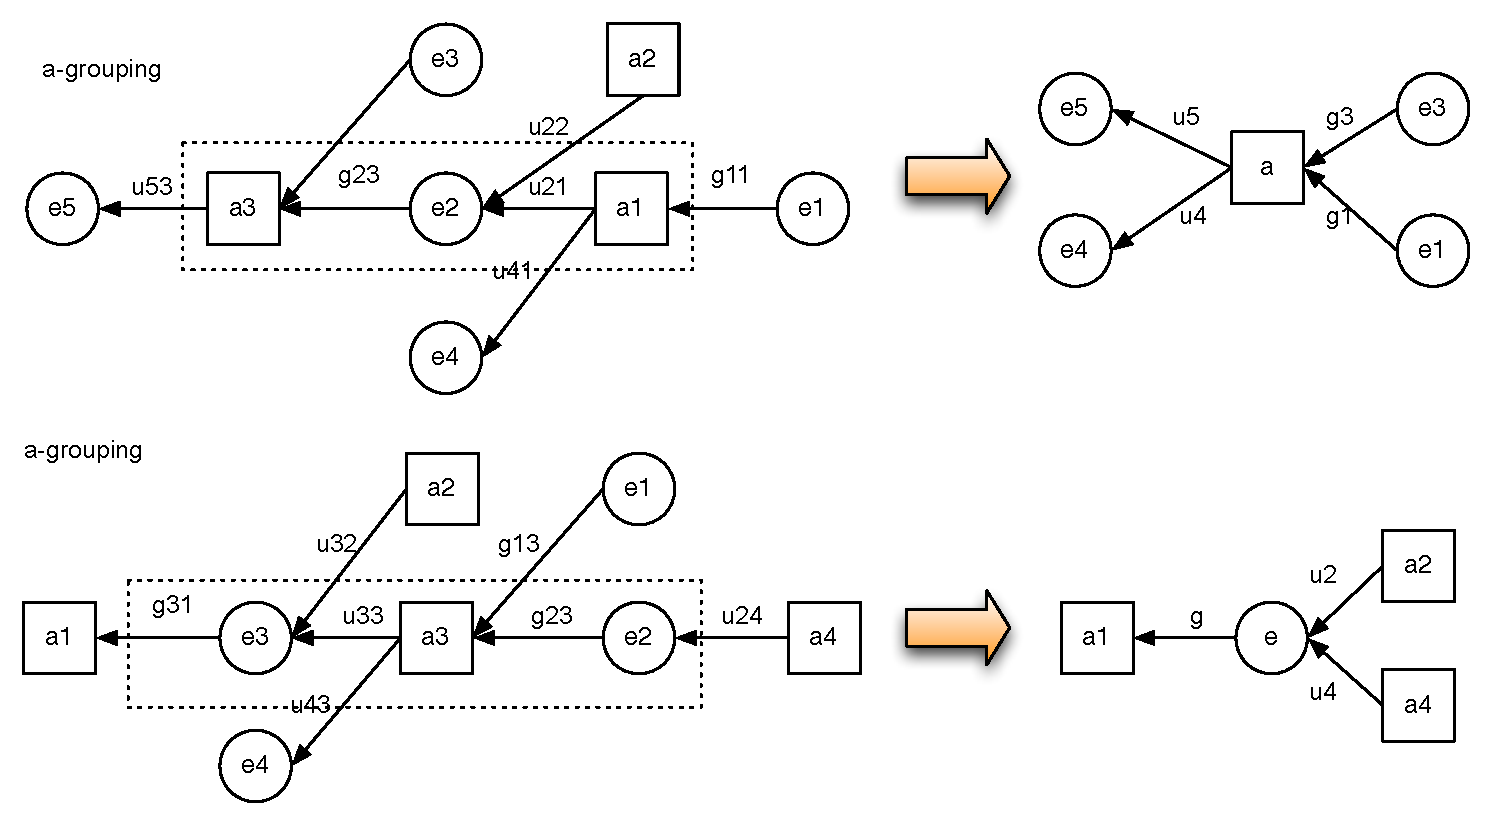
\includegraphics[scale=.5]{figures/a-grouping-pattern-proofs} 
%\caption{$\guEA$ graph patterns for e- and a-grouping} \label{fig:a-grouping-pattern-proofs}
%\end{figure}

% \jwb{
% \subsection{Multiple Applications of Group}
% \label{sec:allowing}
% }
% 
% \comment{replace iterates over all subgroups. this bit not needed. }
% \comment{the most general case produces two or more disjoint subgraphs (where disconnect means there is no path from any node in one to any node in the other  }
% 
% \jwb{In this section we relax the assumption made after Definition~\ref{def:clos}, that the subgraph identified by  $\pclos(V_{gr},G)$ is connected.}
% %
% \jwb{If, instead,  two separate subgraphs are identified within $\pclos(V_{gr},G)$, there are two possibilities. Either following the application of $\extend$ (which extends the set of nodes encompassed) the two subgraphs remain separate, in which case they should be treated as two graphs, or following the applications of $\extend$ the two subgraphs overlap. }
% %
%   \jwb{In this case, we must show that the order in which the $\repl$ functions are carried out is unimportant.}
%   %
%   \jwb{Note that, because it was only at the point of using $\extend$ that the graphs overlapped, we only need to consider the order of application of the two $\repl$ functions.}
% 
% \begin{theorem}\label{thm:multiple}
% \jwb{Let $V_1 \inter V_2 \neq \emptyset$. It is the case that
%    \[
%   \repl(V_1,v_n,\repl(V_2,v_m,G)) =   \repl(V_2,v_m,\repl(V_1,v_n,G))
%   \]}
% \noindent
% \end{theorem}
% \jwb{Proof:~\ref{app:multiple}.}
%

\subsection{Complexity of grouping operators}  \label{sec:complexity}


The grouping operator ensures that the validity of a PROV graph is preserved, that is, the abstracted graph that results from a valid PROV graph does not violate PROV constraints.
Such guarantee, however, comes at a cost which is defined by the complexity of the $\pclos()$ and $\extend()$ operators.
Here we analyse their worst-case complexity, and then argue that much better performance is expected in practical cases.

Firstly, observe that the closure operator can be reduced to a special case of the node reachability problem for acyclic digraphs.
Specifically, given two nodes $v_1, v_2 \in V_{gr}$ such that $v_2$ is reachable from $v_2$, we need to collect all nodes along \textit{all} paths that connect $v_1$ to $v_2$.
This can be accomplished by enumerating all nodes $x$ that are reachable from each $v \in V_{gr}$ while keeping track of the corresponding paths. Whenever $ x \in V_{gr}$, we collect all nodes along the recorded path from $v$ to $x$.

It is easy to see that the worst-case scenario occurs when the nodes in $V_{gr}$ are located at the two ends of the graph, i.e., they are either source or sink nodes.
In such case, the reachability algorithm needs to visit \textit{all} nodes $V$ and \textit{all} edges $E$ in the graph, and it must additionally keep track of all edges it traverses.

Using a simple BFS approach,  we can solve the reachability problem in $O(\mid V\mid + |E|)$ steps, which in the worst-case is $O(|V|^2)$, with a $O(\mid E\mid)$ space complexity for recording all edges. 
Note that the many algorithms that exist to address the problem aim to strike a balance between the cost of pre-processing the graph in order to efficiently answer multiple reachability queries, and the complexity of each individual query.
In our case, however, we can dispense with pre-processing as we expect the closure over $V_{gr}$ to be computed only once.\footnote{Note however that, when consecutive abstraction rounds are envisioned, i.e., abstraction over abstracted graphs, pre-processing may be appropriate, but that needs to be balanced against the cost of updating the data structures after each abstraction round.}

An experimental evaluation of the actual cost of computing closures in practice is beyond the scope of this paper, which is focused on the theoretical underpinnnings of the abstraction operations.
However, two factors suggest that the practical complexity will be considerably less than the worst-case.
Firstly, we can stop the graph traversal as soon as we have visited all $V_{gr}$ nodes. Unless one of those is a sink node, this results in pruning part of the graph. 
Note also that in this case the abstraction will consist of one single abstract node that represents the entire graph, because the closure will include all nodes, which is unlikely to be a desired outcome.
And secondly, in a provenance graph not all edges are allowed, in fact the graph is bipartite with respect of the nodes types (entities and activities), and furthermore, there is at most one generating activity per entity. These factors greatly reduce the expected number of edges to much less than the theoretical max $|V|^2$.

Regarding the $\extend()$ operator, note that this requires all nodes in $\pclos(V_{gr}, G)$ to be visited in order to check their type and possibly extend the closure to their immediate successors. 
This is a linear problem in the worst case, namely when the closure contains all nodes in the graph (in practice, we expect the closure to be much smalller than the graph).


\subsection{Summary}


%\comment{finishing para}
\jwb{In this section we have presented functions that abstract information in a provenance  graph.  We first presented  \emph{homogeneous grouping}  (in Section~\ref{sec:closure}), in which the user selects a set of nodes \emph{of the same type}, and for which the new, abstract node retains that type. Section~\ref{sec:generalisation} extended this to allow the user to select any nodes, at the expense of having to chose the type of the final, abstract, node. Section~\ref{sec:allowing} shows that multiple applications of $\group$ give the same result irrespective of order. 
}

\jwb{It is clear that, in order to meet our initial requirement of maintaining type-correctness of the abstracted graph, more nodes than just the original ones selected will have to hidden. This has implications for the use of this operator, especially given that hidden information may be a critical part of the graph. We address this  problem in~\citep{MBGCD14} where we present a simple policy model and language for controlling abstraction, in the context where provenance owners want to control the disclosure of their provenance graphs. There, the senders define a policy which results in a sensitivity vale being associated with nodes, which gives us a means of evaluating the ``damage'' to a graph caused by the abstraction operator.}

\comment{Address: It is not evident what is the impact of hiding information which the user did not select, especially information that was obfuscated to maintain validity?  What if the non selected obfuscated content is actually the information that must be communicated between the two parties. }

\jwb{Another approach which is open to us following the result of Theorem~\ref{the:multiple} break the initial set chosen by the user into multiple smaller sets, thereby reducing the amount of extra information hidden. This could be taken to its logical limit by abstracting individual nodes, but this  would have to be balanced  against the increasing revelation of the structure of the graph.  A full investigation of this is beyond the scope of this paper.
  }



\jwb{In the following section we evaluate the consistency of the abstractions we propose on the ordering constraints C2-C7. }
